
\chapter{System description}

This chapter will describe how the inverter and genset are constructed to get a better understanding of the system. 

\section{Inverter}
This section will contain an introduction to the inverter.

\subsection{Grid-connected PV inverter}
\label{PVinverter}

During the application of PV inverters the main task is to convert PV power provided by the solar panels in DC voltage to AC, stabilize the output voltage, frequency and current, and feed power to the utility grid. When the inverter works parallel to the genset, the main task is to deliver power according to the reference provided by the ASC. Furthermore the power should be delivered at the voltage and frequency provided by the genset, the inverter should therefore always match this.
A typical diagram of a grid connected PV system can be seen in \figref{fig:gridPV}.    
\begin{figure}[H]
\begin{tikzpicture}
    \coordinate (SolarCellP) at (0.5,0);
    \coordinate (ChopperP) at (4,0);
    \coordinate (InverterP) at (8,0);

    % Place blocks
    \begin{scope}[every node/.style={draw,thick, fill=white!30, rectangle,text width=1.5cm, minimum height=2cm, text badly centered}]
        \node[name=pv,pattern=grid,pattern color=white!30] at (SolarCellP) { PV};
        \node[name=chopper] at (ChopperP) {DC/DC};
        \node[name=inverter] at (InverterP) {DC/AC};
    \end{scope}

    \draw
    % PV to chopper
        (pv.30) -- (chopper.150)
        (pv.330) -- (chopper.210)
    % DC link and cap
        (chopper.30) -- (inverter.150)
        (chopper.330) -- (inverter.210)
        ($(chopper.330)!0.4!(inverter.210)$) to[capacitor, l=\SI{}{}, mirror] ($(chopper.30)!0.4!(inverter.150)$)
    % AC side
        (inverter.30)
        to[L] ++(1.1,0)
        %to[short] ++(1,0)
        to[L] ++(1.1,0)
        to[short] ++(1,0) coordinate(N1)
        to[short] ++(1,0)  %line
        |- (inverter.330)
        % ------------------------ Secondary side
        (N1)++(0.65,0) coordinate (N2)
            %to[open] ($(N2)+(0,-1)$)
            %to[short] (N2)
            %to[short] ++(1,0)
            to[sV, l=$Grid$] ++(0,-1)
            %to[short] ++(-1,0)
    ;
    \draw ($(inverter.330)+(1.1,0)$) to[C] ++(0,1.033);
    \draw[thick,dashed] ($(-1.5,-1.5)+(chopper)$) -- ($(-1.5,2)+(chopper)$) -- ($(3.1,2)+(inverter)$) -- ($(3.1,-1.5)+(inverter)$) -- ($(-1.5,-1.5)+(chopper)$);
    \node[] at ($(2.5,1.5)+(chopper)$) {\textbf{Inverter}};
\end{tikzpicture}
\caption{Grid-connected PV system.}
\label{fig:gridPV}
\end{figure}

As can be seen in \figref{fig:gridPV} the system usually consists of a boost (DC/DC) converter which scales up the output voltage of the PV to a certain DC level. According to the available power, usually an algorithm called MPPT (Maximum Power Point Tracker) controls the output current and voltage in such a way that the output power is the maximum possible. The DC/AC inverter provides a 3-phase (or in some cases 1-phase) voltage and current signals, therefore the energy from a solar cell can be utilized and transported to the utility grid. 

In order to create sinusoidal voltage on the output, usually LC or LCL filters are applied that dampen the high frequency peaks and leaving only the lower frequencies in the inverter output. 

\subsection{General inverter concepts}
\label{inverter}

In the presented project an inverter from SMA with model number STP20000 of the Pulse Width Modulation(PWM)-type was provided. This kind of unit is capable of creating both active- and reactive-power from 3-phase voltages and currents in accordance with the load on the system. Although the control for such electronic devices can vary in a wide range, there are existing several schemes to generate AC voltage from DC via PWM. Out of several techniques, a scheme called sinusoidal pulse width modulation (SPWM) is assumed and will be discussed, as the outcome of other schemes would be similar and the SPWM scheme provides a basic understanding of the working principle.

Despite the fact that the project deals with a 3-phase inverter, it is sufficient to introduce the basic concepts of operation in a 1-phase example.
A basic hardware structure for PWM control is a H-bridge as seen in \figref{fig:inverterblock}. More advanced and sophisticated structures are more likely used in the provided inverter, as these improve both efficiency, noise canceling and leakage currents, however the principle for these does not differ significantly. \cite{aau_invert_topologies}. 


\begin{figure}[H]
\centering
\begin{circuitikz}[thin,scale=1, every node/.style={scale=0.78}]
% TRANSISTORS
\draw
(0,2) node[pigfete] (t1) {}
(0,0) node[nigfete] (t2) {}
(2,2) node[nigfete] (t3) {}
(2,0) node[nigfete] (t4) {};
\draw
(t1.S) to[short] (t2.D)
(t3.S) to[short] (t4.D);
% DIODES and transistor labels
\foreach \num in {1,2,3,4} {
\node[anchor=south] at (t\num.G) {$T_\num$};
\draw (t\num.S)++(0,0.5) -- ++(0.3,0) to[sD*] ($(t\num.D)+(0.3,-0.5)$) -- ++(-0.3,0);
}          
% BATTERY connection
\draw
(t4.S) to[short,-*] (t2.S) to[short] ($(t2.S)+(-2,0)$)
to[battery,l=$U$] ($(t1.D)+(-2,0)$) to[short,-*] (t1.D) to[short] (t3.D);
% RL
\draw
(t1.S) to[short,*-] ($(t1.S)+(3,0)$) to[short] ($(t1.D)+(3,0)$) coordinate (p1)
to[R,l_=$R$] ++(2,0) to[L,l_=$L$,i>^=$i_L$] ++(3,0) coordinate (p);
\draw
(t4.D) to[short,*-] ($(t4.D)+(1,0)$) to[short] ($(t4.S)+(1,0)$) coordinate (n1)
to[short] ++(5,0) coordinate (n);
% C
\draw
(p) to[C,l=$C$,i>^=$i_C$,v<=$U_C$] (n);
% LOAD
\draw
(p) to[short,*-]($(p)+(2,0)$) to[R,l=$LOAD$,i>^=$i_o$] ($(n)+(2,0)$) to[short,-*] (n);
% U_i
\draw
(p1) to[open,v^=$U_i$] (n1);

\end{circuitikz}
\caption{Full-bridge inverter with load}
\label{fig:inverterblock} 
\end{figure}
 
Most of the inverters usually deal with a full-bridge topology consisting of MOSFETs or IGBTs. The 1-phase circuit illustrated in \figref{fig:inverterblock} has four semiconductor switches with protection diodes, making it possible to create both current and voltage signals with controllable magnitude and frequency, thus controllable active and reactive power components. Each of these switches are controlled by the modulated control signal, namely $T_1$ and $T_4$ with $S$ while $T_2$ and $T_3$ with  $\neg{S}$ which is the negated signal of $S$.

The scheme of modulating $S$ can be seen in \figref{fig:sinPWM} where a sine (control signal - $V_{control}$) and a triangular (reference signal - $V_{tri}$) are compared.   

\begin{figure}[H]
\centering
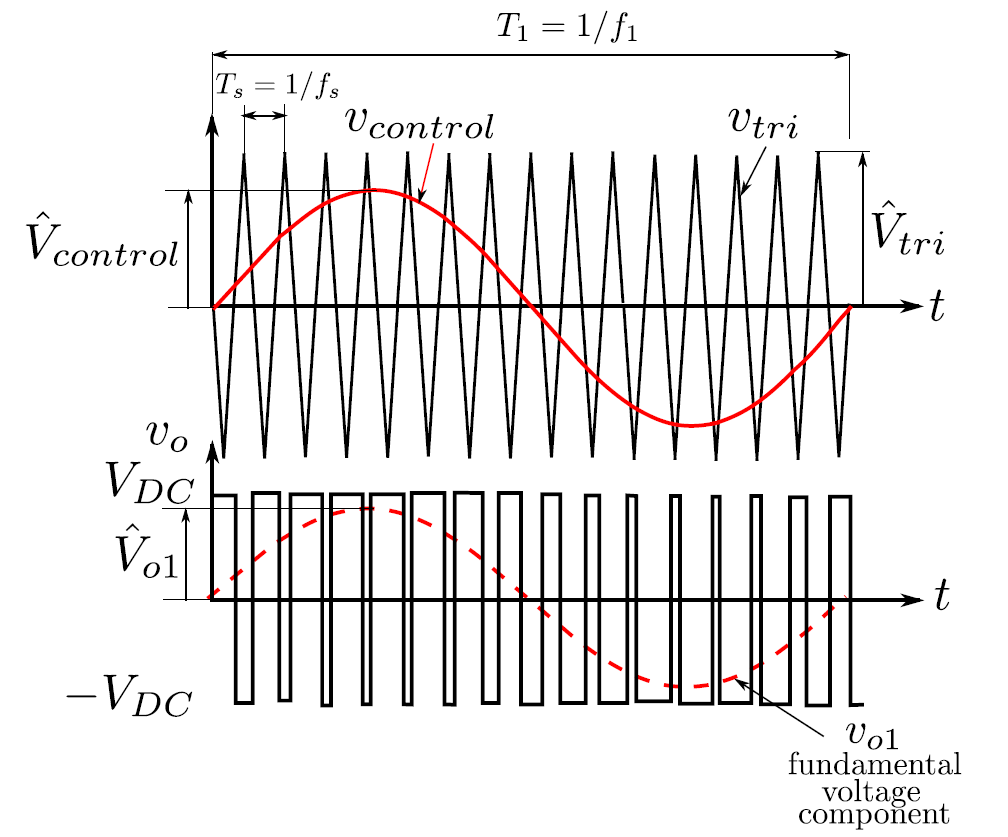
\includegraphics[width=0.6\textwidth]{rapport/analyse/sinPWM}
\caption{Sinusoidal PWM \cite{bud_inverter_PV}}
\label{fig:sinPWM}
\end{figure}

As can be seen, there are two cases given. When 
\begin{equation} 
\label{eq:case1}
V_{control} > V_{tri} %\unit{W}
\end{equation}
then $T_1$ and $T_4$ are conducting, thus switching the DC voltage coming from the PV, while $T_2$ and $T_3$ are turned off. However, when 
\begin{equation} 
\label{eq:case1}
V_{control} < V_{tri}
\end{equation}
then $T_2$ and $T_3$ are conducting and switching $V_{DC}$ therefore $T_1$ and $T_4$ are turned off. As can be seen, this switching pattern results in a PWM output signal with a sinusoidally varying duty cycle. While the output voltage is a square signal, the output current can result in an almost perfectly sinus wave(according to the load on the system) if the switching frequency is sufficiently high. Thus, as mentioned previously usually an LC or LCL filter is applied to the inverter voltage output in order to dampen the high frequency components. 

The frequency of the desired output voltage can be determined by the frequency of the control signal $f_1$ which is the fundamental component of the waveform. The switching frequency equals to the frequency of $V_{tri}$, while the magnitude of the triangular waveform is usually kept constant in order to simplify the control of the voltage and frequency. Therefore the two modulation indexes can be given as: 
\begin{equation} 
\label{eq:ma}
m_a = \frac{\tilde{V}_{control}}{\tilde{V}_{tri}}
\end{equation}
\begin{equation} 
\label{eq:mf}
m_f = \frac{f_1}{f_s}
\end{equation}

where $\tilde{V}_{control}$ and $\tilde{V}_{tri}$ are magnitudes of the signals.

As can be seen from the relations, the controller of the inverter should measure frequency and voltage of the output waveforms at the same time to modify $m_a$ and to align the desired frequency by adjusting $m_f$.

\section{Diesel Generator}
\label{diesel_generator}
This section will contain an introduction to the diesel generator.

Gensets are used to provide electrical power in areas where utility electricity is not available, or when electricity is only needed temporarily or in situations when the power grid fails due to power plant breakdowns. Gensets are also used in isolated places where there is no grid.
In case of these isolated areas, when there is no grid, a specificied amount of frequency and voltage should be delivered to a non-stiff grid. The name of this operation is called island mode. 

A genset is a system which is a combination of a diesel engine and an electric generator which converts mechanical energy into electrical. Gensets consist of several subsystems, starting from the engine, generator, governor and the AVR \cite{genset_how_it_works}. These subsystems are illustrated in \figref{fig:genset_blockdiagram}.  
 
\begin{figure}[H]
\centering
\includegraphics[width=0.75\textwidth]{rapport/billeder/genset_blockdiagram}
\caption{Block diagram of a genset showing the engine, the generator and their controllers.}
\label{fig:genset_blockdiagram}
\end{figure}

The diesel engine is the source of mechanical energy, therefore provides input to the generator. It delivers a specific amount of rounds per minute (RPM) which is controlled by the governor. When the RPM decreases, which will happen when there is an increase in load, the governor adjusts according to the disturbance and injects more fuel into the engine to deliver more mechanical power into the electric generator and vice versa when the load decreases. 

The electric generator consists of an alternator which task is to produce the electrical power when it is driven by the diesel engine \cite{genset_how_it_works}.

\begin{figure}[H]
\centering
\includegraphics[width=0.75\textwidth]{rapport/billeder/statorrotor}
\caption{Illustration of the rotor and the stator inside the shell \cite{rotor_stator_pic}.}
\label{fig:statorrotor}
\end{figure}

The alternator consists of two different parts: the stator and the rotor. The stator is the stationary component which is fixed inside the alternators shell and the rotor creates (when it is driven within the stator) a magnetic field that conducts a current in the windings of the stator \cite{genset_how_it_works}. The alternating voltage regulator (AVR) regulates the induced voltage in the stator windings therefore attempts to keep it at a constant level. 

These two control schemes for the governor and the AVR are usually referred to as isochronous and are based on PID algorithms. 
 

In \secref{modelling_diesel_generator} a TF for a genset will be derived.  

%As it was mentioned in the system description, the governor is responsible for the fuel injection, 
%while the regulation of the induced voltage in the stator windings is handled by the AVR. In the model of the genset,
% the AVR and the governor use a control scheme called isochronous, based on simple PID algorithms.





